
% -------------------------------------------
% Items to substitute into the ivoatex document template.
%
%\ivoagroup{Data Model Working Group}

%\title{Astronomical Measurements Model}


%\author{Arnold Rots}
    
%\author{Mark Cresitello-Dittmar}
    
%\author{Omar Laurino}
    
%\previousversion{0.x}
      
% -------------------------------------------

\pagebreak
\section{Model: meas }
  
  % INSERT FIGURE HERE
  \begin{figure}[h]
  \begin{center}
    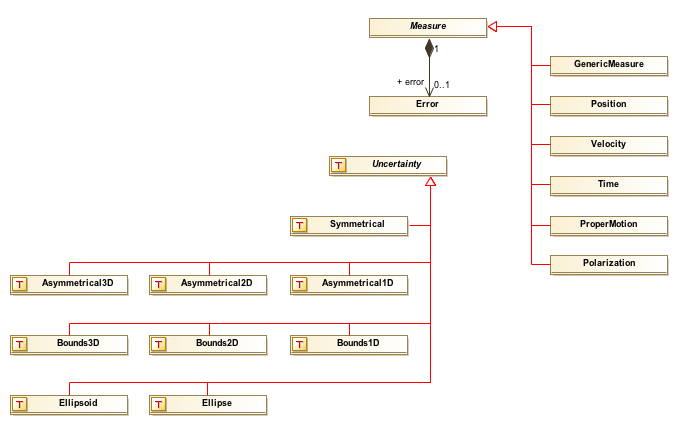
\includegraphics[width=5.75in]{diagrams/Overview.png}
    \caption{Overview of Measurement model elements}\label{fig:overview}
  \end{center}
  \end{figure}

  This model defines objects and datatypes which represent 'measured' or 'determined' data. It associates a Coordinate (ie: the determined value with associated physical context) with corresponding Error(s). As such, this model is at least the foundation for representing the vast majority of the Astronomical data found in catalogs and data products. 

We define here, several specialized classes which cover the most basic and common types, such as Position and Time. We also provide a generic model which can accommodate virtually any data, but may require a bit more effort to fully describe the coordinate metadata. Additional specializations, e.g. Flux, Magnitude, Luminosity, Pressure, Temperature, etc. may be added to this model, or in other models focusing on particular domains or use cases. 

We include a fairly simple Error model, describing errors as a 'shape' of uncertainty, and define a small set of commonly occuring forms (e.g. Symmetrical, Bounds, Ellipsoid).

\pagebreak
\section{Measure}

  % INSERT FIGURE HERE
  \begin{figure}[h]
  \begin{center}
    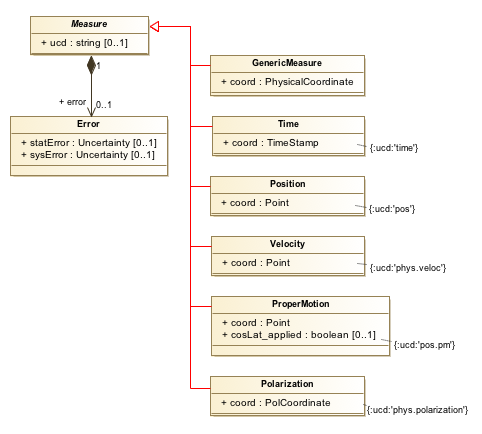
\includegraphics[width=3.5in]{diagrams/Measure.png}
    \caption{Measure elements}\label{fig:measure}
  \end{center}
  \end{figure}

  \subsection{Measure (Abstract)}
  \label{sect:Measure}
    Abstract base of Measure classes, associates a 'determined value' (Coordinate) with corresponding errors. We associate the Error(s) with the full Measure, rather than the individual values, in order to support both correlated and uncorrelated errors. In many cases with multi-dimensional data, the associated errors are correlated and must be considered with the value set as a whole. One consequence of this approach is that there is a looser association between the Error dimensions and the corresponding value dimension. We require that the Error content MUST be compatible with the value dimension and nature (e.g. dimension, domain, units, etc).

    \subsubsection{Measure.error}
      \textbf{vodml-id: Measure.error} \newline
      \textbf{type: \hyperref[sect:Error]{meas:Error}} \newline
      \textbf{multiplicity: 0..1} \newline 
      Measurement error.

  \subsection{Error}
  \label{sect:Error}
    The Error class uses the Uncertainty types to describe measurement errors from various sources.

    \subsubsection{Error.statError}
      \textbf{vodml-id: Error.statError} \newline
      \textbf{type: \hyperref[sect:Uncertainty]{meas:Uncertainty}} \newline
      \textbf{multiplicity: 0..1} \newline 
      Statistical error. The Uncertainty type MUST be dimensionally compatible with the associated Measure value.

    \subsubsection{Error.sysError}
      \textbf{vodml-id: Error.sysError} \newline
      \textbf{type: \hyperref[sect:Uncertainty]{meas:Uncertainty}} \newline
      \textbf{multiplicity: 0..1} \newline 
      Systematic error. The Uncertainty type MUST be dimensionally compatible with the associated Measure value.

    \subsubsection{Error.ranError}
      \textbf{vodml-id: Error.ranError} \newline
      \textbf{type: \hyperref[sect:Uncertainty]{meas:Uncertainty}} \newline
      \textbf{multiplicity: 0..1} \newline 
      Random error. The Uncertainty type MUST be dimensionally compatible with the associated Measure value.


  \subsection{GenericMeasure}
  \label{sect:GenericMeasure}
    The most generic Measure class. This class may be used to represent data not covered by the specialized cases.

    \subsubsection{GenericMeasure.coord}
      \textbf{vodml-id: GenericMeasure.coord} \newline
      \textbf{type: coords:PhysicalCoordinate} \newline
      \textbf{multiplicity: 1} \newline 
      The measured coordinate value.

  \subsection{Time}
  \label{sect:Time}
    Provides a complete description of a measured Temporal instant.

    \subsubsection{Time.coord}
      \textbf{vodml-id: Time.coord} \newline
      \textbf{type: coords:TimeStamp} \newline
      \textbf{multiplicity: 1} \newline 
      The measured time value. May be provided in any of the TimeStamp subtypes.


  \subsection{Position}
  \label{sect:Position}
    Provides a complete description of a measured positional instant.

    \subsubsection{Position.coord}
      \textbf{vodml-id: Position.coord} \newline
      \textbf{type: coords:Point} \newline
      \textbf{multiplicity: 1} \newline 
      The measured Position value. The Point coordinate supports 1,2, and 3-dimensional cases. Details of the coordinate system (space and frame), are associated with the Point.


  \subsection{Velocity}
  \label{sect:Velocity}
    Provides a comple description of a measured Velocity instant.

    \subsubsection{Velocity.coord}
      \textbf{vodml-id: Velocity.coord} \newline
      \textbf{type: coords:Point} \newline
      \textbf{multiplicity: 1} \newline 
      The measured Velocity value. The Point coordinate supports 1,2, and 3-dimensional cases. Details of the coordinate system (space and frame), are associated with the Point.


  \subsection{ProperMotion}
  \label{sect:ProperMotion}
    Proper motion represented as the velocity in Longitude and Latitude directions of a spherical coordinate space. The associated SpaceFrame provides the details regarding the nature of the coordinate space (eg: Equatorial, Galactic, etc).

    \subsubsection{ProperMotion.lon}
      \textbf{vodml-id: ProperMotion.lon} \newline
      \textbf{type: coords:PhysicalCoordinate} \newline
      \textbf{multiplicity: 1} \newline 
      Velocity in angular distance per unit time along the Longitude axis. It is common, though not universal, practice to quote longitudinal proper motion pre-multiplied by cos(lat) so that the magnitude of the quantity is not affected by its longitudinal position. We do not constrain this value to one form or the other in this model, leaving it to be specified by the particular usage thread.

    \subsubsection{ProperMotion.lat}
      \textbf{vodml-id: ProperMotion.lat} \newline
      \textbf{type: coords:PhysicalCoordinate} \newline
      \textbf{multiplicity: 1} \newline 
      Velocity in angular distance per unit time along the Latitude axis.

  \subsection{Polarization}
  \label{sect:Polarization}
    Provides a complete description of a determined polarization state. Since the polarization coordinate is an enumerated type, there can be no associated numerical error sources.

    \noindent \textbf{constraint} \newline
    \indent    \textbf{detail: Polarization.error:Error[0] }\newline


    \subsubsection{Polarization.coord}
      \textbf{vodml-id: Polarization.coord} \newline
      \textbf{type: coords:PolCoordinate} \newline
      \textbf{multiplicity: 1} \newline 
      Determined polarization state. May be provided by any of the PolCoordValue subtypes.

\pagebreak
\section{Uncertainty}

  % INSERT FIGURE HERE
  \begin{figure}[h]
  \begin{center}
    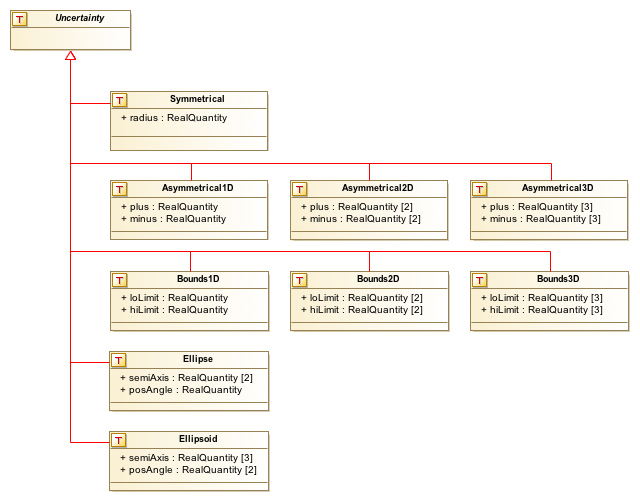
\includegraphics[width=5in]{diagrams/Uncertainty.png}
    \caption{Uncertainty elements}\label{fig:uncertainty}
  \end{center}
  \end{figure}

  \subsection{Uncertainty (Abstract)}
  \label{sect:Uncertainty}
    Abstract head of uncertainty types. These classes define the shape of the uncertainty, and are designed to be reusable in different contexts. Uncertainties are designed to be associated with a Coordinate or other object which provides the 'center' or reference location about which the uncertainty resides. 

In this model, we use them in the context of defining measurement errors, but they are also compatible for use in defining resolutions which are to be modeled at a later date. This initial version of teh model forms a fundamental basis which can then be expanded to include more complex and varied use cases as they present themselves. The current model assumes Gaussian distributions with shpes defined at the 68\% confidence level.

  \subsection{Symmetrical}
  \label{sect:Symmetrical}
    Symmetrical uncertainty, constant in all dimensions and directions from the associated Coordinate. ie: PlusMinus in 1D, circular in 2D, spherical in 3D.

    \subsubsection{Symmetrical.radius}
      \textbf{vodml-id: Symmetrical.radius} \newline
      \textbf{type: \hyperref[sect:ivoa]{ivoa:RealQuantity}} \newline
      \textbf{multiplicity: 1} \newline 
      The uncertainty extent, constant in all dimensions and directions.

  \subsection{Asymmetrical1D}
  \label{sect:Asymmetrical1D}
    Uncertainty with different extent in the positive and negative directions from the associated Coordinate.

    \subsubsection{Asymmetrical1D.plus}
      \textbf{vodml-id: Asymmetrical1D.plus} \newline
      \textbf{type: \hyperref[sect:ivoa]{ivoa:RealQuantity}} \newline
      \textbf{multiplicity: 1} \newline 
      Extent in the positive axis direction.

    \subsubsection{Asymmetrical1D.minus}
      \textbf{vodml-id: Asymmetrical1D.minus} \newline
      \textbf{type: \hyperref[sect:ivoa]{ivoa:RealQuantity}} \newline
      \textbf{multiplicity: 1} \newline 
      Extent in the negative axis direction.

  \subsection{Asymmetrical2D}
  \label{sect:Asymmetrical2D}
    2D Uncertainty with different extent in the positive and negative axis directions from the associated Coordinate. i.e.: an offset rectangle.

    \subsubsection{Asymmetrical2D.plus}
      \textbf{vodml-id: Asymmetrical2D.plus} \newline
      \textbf{type: \hyperref[sect:ivoa]{ivoa:RealQuantity}} \newline
      \textbf{multiplicity: 2} \newline 
      Extent in each positive axis direction.

    \subsubsection{Asymmetrical2D.minus}
      \textbf{vodml-id: Asymmetrical2D.minus} \newline
      \textbf{type: \hyperref[sect:ivoa]{ivoa:RealQuantity}} \newline
      \textbf{multiplicity: 2} \newline 
      Extent in each negative axis direction.

  \subsection{Asymmetrical3D}
  \label{sect:Asymmetrical3D}
    3D Uncertainty with different extent in the positive and negative axis directions from the associated Coordinate. i.e.: an offset box.

    \subsubsection{Asymmetrical3D.plus}
      \textbf{vodml-id: Asymmetrical3D.plus} \newline
      \textbf{type: \hyperref[sect:ivoa]{ivoa:RealQuantity}} \newline
      \textbf{multiplicity: 3} \newline 
      Extent in each positive axis direction.

    \subsubsection{Asymmetrical3D.minus}
      \textbf{vodml-id: Asymmetrical3D.minus} \newline
      \textbf{type: \hyperref[sect:ivoa]{ivoa:RealQuantity}} \newline
      \textbf{multiplicity: 3} \newline 
      Extent in each negative axis direction.

  \subsection{Bounds1D}
  \label{sect:Bounds1D}
    Provide the edges of the uncertainty space. Rather than being relative to the associated Coordinate, these represent a range within that Coordinate space.

    \subsubsection{Bounds1D.loLimit}
      \textbf{vodml-id: Bounds1D.loLimit} \newline
      \textbf{type: \hyperref[sect:ivoa]{ivoa:RealQuantity}} \newline
      \textbf{multiplicity: 1} \newline 
      Lower limit of the uncertainty range.

    \subsubsection{Bounds1D.hiLimit}
      \textbf{vodml-id: Bounds1D.hiLimit} \newline
      \textbf{type: \hyperref[sect:ivoa]{ivoa:RealQuantity}} \newline
      \textbf{multiplicity: 1} \newline 
      Upper limit of the uncertainty range.

  \subsection{Bounds2D}
  \label{sect:Bounds2D}
    Provide the edges of a 2D uncertainty space. Rather than being relative to the associated Coordinate, these represent ranges along each axis of that Coordinate space.

    \subsubsection{Bounds2D.loLimit}
      \textbf{vodml-id: Bounds2D.loLimit} \newline
      \textbf{type: \hyperref[sect:ivoa]{ivoa:RealQuantity}} \newline
      \textbf{multiplicity: 2} \newline 
      Lower edges of the uncertainty rectangle.

    \subsubsection{Bounds2D.hiLimit}
      \textbf{vodml-id: Bounds2D.hiLimit} \newline
      \textbf{type: \hyperref[sect:ivoa]{ivoa:RealQuantity}} \newline
      \textbf{multiplicity: 2} \newline 
      Upper edges of the uncertainty rectangle.

  \subsection{Bounds3D}
  \label{sect:Bounds3D}
    Provide the edges of a 3D uncertainty space. Rather than being relative to the associated Coordinate, these represent ranges along each axis of that Coordinate space.

    \subsubsection{Bounds3D.loLimit}
      \textbf{vodml-id: Bounds3D.loLimit} \newline
      \textbf{type: \hyperref[sect:ivoa]{ivoa:RealQuantity}} \newline
      \textbf{multiplicity: 3} \newline 
      Lower edges of the uncertainty box.

    \subsubsection{Bounds3D.hiLimit}
      \textbf{vodml-id: Bounds3D.hiLimit} \newline
      \textbf{type: \hyperref[sect:ivoa]{ivoa:RealQuantity}} \newline
      \textbf{multiplicity: 3} \newline 
      Upper edges of the uncertainty box.

  \subsection{Ellipse}
  \label{sect:Ellipse}
    Elliptical uncertainty shape.

    \subsubsection{Ellipse.semiAxis}
      \textbf{vodml-id: Ellipse.semiAxis} \newline
      \textbf{type: \hyperref[sect:ivoa]{ivoa:RealQuantity}} \newline
      \textbf{multiplicity: 2} \newline 
      Extent of the semi-major and semi-minor axes, provided in the order of the associated Coordinate axes.

    \subsubsection{Ellipse.posAngle}
      \textbf{vodml-id: Ellipse.posAngle} \newline
      \textbf{type: \hyperref[sect:ivoa]{ivoa:RealQuantity}} \newline
      \textbf{multiplicity: 1} \newline 
      Position angle, counter-clockwise from the positive direction of the first axis of the associated Coordinate. When used in the spatial domain, the expectation is that the 'first axis' corresponds to the 'North Celestial Pole', and the second to 'East', thereby conforming to the IAU definition of the position angle direction being 'East of North'.

  \subsection{Ellipsoid}
  \label{sect:Ellipsoid}
    Ellipsoidal uncertainty shape.

    \subsubsection{Ellipsoid.semiAxis}
      \textbf{vodml-id: Ellipsoid.semiAxis} \newline
      \textbf{type: \hyperref[sect:ivoa]{ivoa:RealQuantity}} \newline
      \textbf{multiplicity: 3} \newline 
      Extent of the semi axes, provided in the order of the associated Coordinate axes.

    \subsubsection{Ellipsoid.posAngle}
      \textbf{vodml-id: Ellipsoid.posAngle} \newline
      \textbf{type: \hyperref[sect:ivoa]{ivoa:RealQuantity}} \newline
      \textbf{multiplicity: 2} \newline 
      Position angles
      \begin{enumerate}
      \item counter-clockwise from the positive direction of the first axis toward the second axis
      \item angle 'above' the plane of the first two axes of the associated Coordinate
      \end{enumerate}
      When used in the spatial domain, the expectation is that the 'first axis' corresponds to the 'North Celestial Pole', and the second to 'East', thereby conforming to the IAU definition of the position angle direction being 'East of North'.
